\chapter{Setup}

Hereafter is an image depicting the high level structure of the LORNA project.

\begin{figure}[ht]
    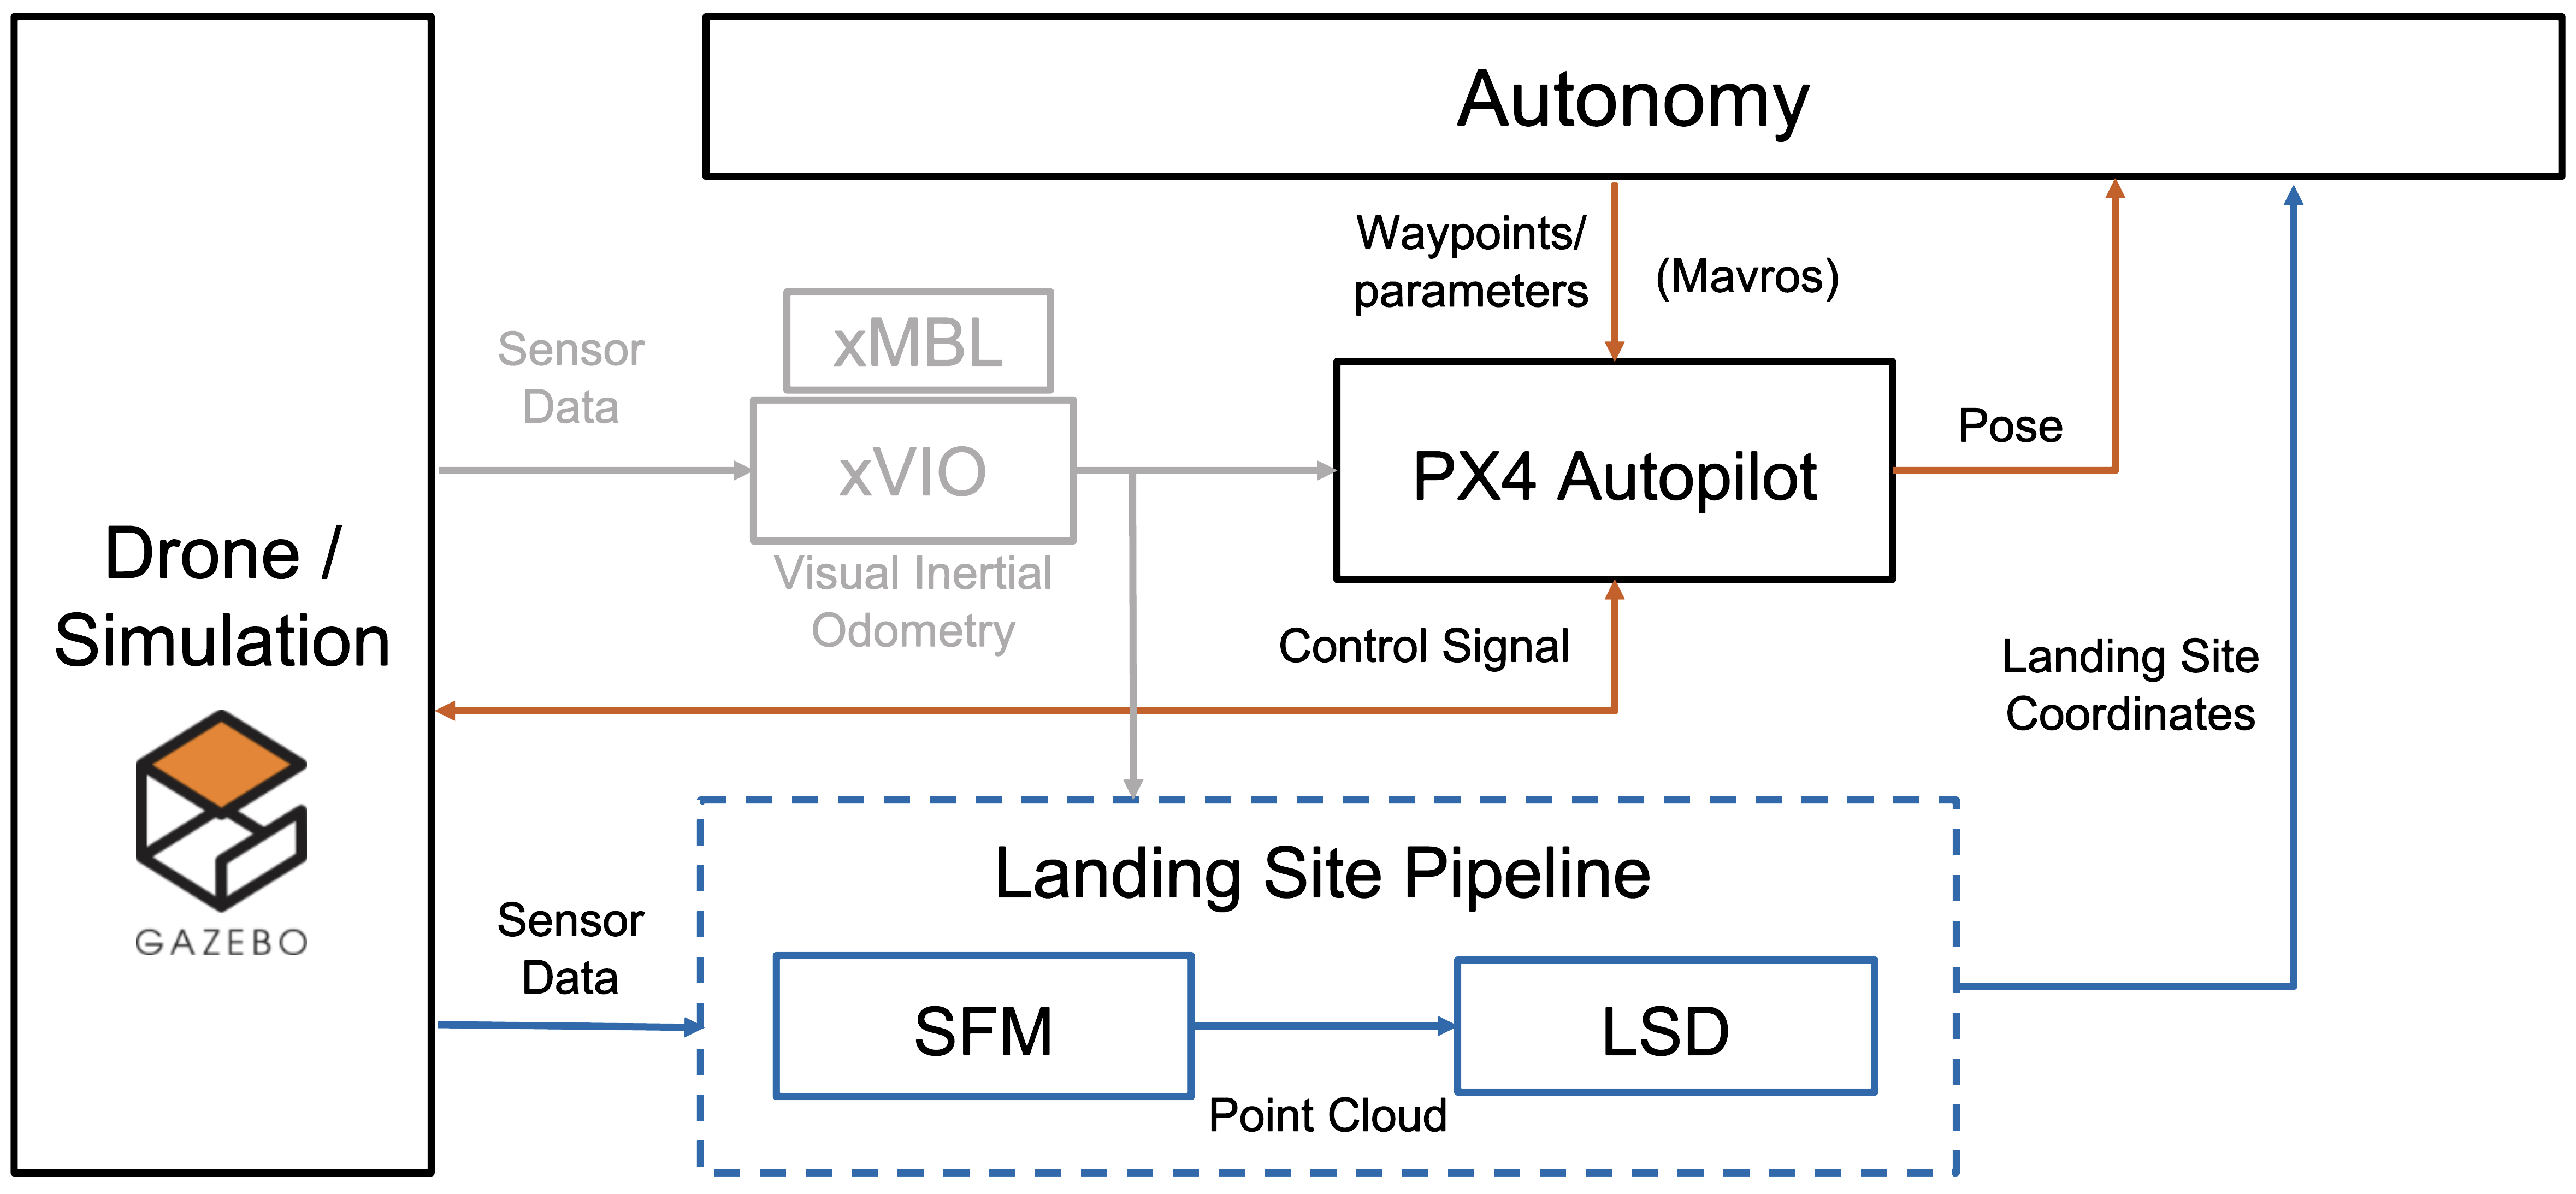
\includegraphics[scale=0.18]{images/setup/setup_flowchart.png}
    \caption{LORNA Project Setup}
    \label{fig:lorna_setup}
\end{figure}

As this thesis revolved around the combination of existing software instances, it is essential to display the individual parts comprising the LORNA project in more detail.

\clearpage %HERE
\section{Simulation}

Despite being able to deploy the landing site detection pipeline onto the voxl2 processor the majority of this thesis was done using a Gazebo Garden simulation of the drone. 

\begin{figure}[ht!]
    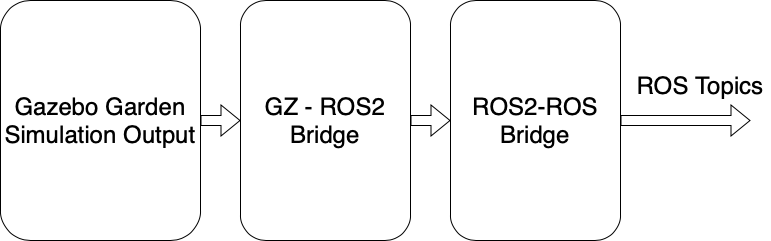
\includegraphics[scale=0.45]{images/setup/GZ_flowchart.png}
    \caption{Gazebo ROS Bridge}
\end{figure}


As the entire software stack of the LORNA project is dependent on ROS instead of ROS2 a bridge was used to convert the sensor information from Gazebo to ROS2 and from ROS2 to ROS.


\section{Landing Site Acquisition Pipeline}\label{sec:setup:LSD}

The landing site acquisition pipeline consists of two nodes. A structure from motion node \citep{SFM} which creates a pointcloud using a keyframe based stereo approach on monocular images and a landing site detector node \citep{LSD1, LSD2} which aggregates the depth measurements into a rolling buffer based multi-resolution depth map and segments landing sites on the created DEM. The found landing sites are then supplied to the autonomy. 

\subsection{Structure From Motion}\label{subsec:setup:SFM}

\subsubsection{SFM - Bundle Adjustment}



In a first step the keyframes are filled with the incoming images and their respective camera pose information. Once the keyframes are filled each iteration the input as well as all the keyframe poses are refined using a Bundle Adjustment algorithm. 

\subsubsection{SFM - Stereo Depth}

The keyframes and their refined poses are then compared to the new incoming image with regards to image overlap and feature retention. Chosing the most adequate keyframe and the incoming frame one can create a depth image. The depth image is then converted into a pointcloud and packaged together with the respective poses of the images. This allows to not only locate that depth information in a given frame but also to derive the baseline with which that pointcloud was created.

\subsection{Landing Site Detection (LSD)}\label{subsec:setup:LSD}

\subsubsection{LSD - Depth Aggregation}

The foundation of the landing site detection mechanism is a rolling buffer based multi resolution depth map. Each cell in this dense elevation map (DEM) contains an optimal mixture of gaussian (OMG) state as described in \citet{LSD2}. Each point cloud input iteration, the measurements are placed in the respective cells based on the level of detail of the perceived points. In a subsequent step the measurements are pooled up and down the resolution layers in order to make the DEM more consistent.

\subsubsection{LSD - Landing Site Segmentation}

On the created depth map landing sites can then be detected. This is done using a roughness and slope assessment of the perceived terrain. Roughness defines the maximum absolute altitude difference around a cell in a certain resolution layer and slope is determined by fitting a plane to the vicinity of a considered point.

If the roughness and slope values lie within the acceptance threshold the landing sites are selected as such in a binary landing map. After applying a distance transform and performing non-maximum suppression the biggest landing sites are found. These are then refined one last time using a mean shift algorithm that considered roughness, slope and size once again.


\section{Autonomy}\label{sec:setup:autonomy}

The autonomous framework was developed within the LORNA project. It is the overarching instance governing all the necessary behaviors and constituting the interface between all the different nodes of the process. It is connected to the flight controller through the Mavros wrapper of the Mavlink protocol. With this connection it can send waypoints and parameter updates to the flight controller.
In addition to the in \cref{fig:lorna_setup} shown connections it also communicates with a healthguard node keeping track of the systems health state and alerting in case of anomalies.
% TODO








